According to \citeauthor{Keim2010}, visual analytics "[\ldots] is not easy to define, due to its multi-disciplinary nature involving multiple processes and the wide variety of application areas \iacite{Keim2010}." Based on current practice, they define visual analytics as the combination of automated anlysis techniques with interactive visualisatoins for an effective understanding, reasoning and decision making on the vasis of very large and complex datasets \iacite{Keim2010}.

So, based on the definition, \citeauthor{Keim2010} elaborate the objectives of visual analytics to state that it is the creation of tools and techniques to enable people to:

\begin{itemize}
\item Summarize information and derive insight from heterogeneous and often conflicting data.
\item Detect the expected and discover the unexpected.
\item Provide reasonable and understandable evaluations.
\item Communicate these evaluations effectively for action.
\end{itemize}

The following part in this chapter gives an overview of how visual analytics tries to achieve these objectives to generate knowledge from data. Thereafter a look on the many scientific disciplines that contribute to visual analytics is made.
Based upon that knowledge gathered in this chapter and the chapters before, it is possible to derive design principles for good visualizations.

Figure \ref{fig:va-process} on page \pageref{fig:va-process} shows an abstract overview of the visual analytics process. It contains different stages, represented as colored ovals, and their corresponding transitions, represented as arrows. The first step of the process deals with the integration of heterogeneous data sources. This integration includes tasks like data preprocessing, transforming, cleaning, normalization, grouping and fusion. All those tasks are indicated by the transformation transition onto the data oval. After the transformation, the analyst has two different options to choose \iacite{Keim2010}:

\begin{enumerate}
\ditem{Automated data analysis} \hfill \\
If an automated model was chosen first, data mining methods are applied to generate statistical models out of the original data. Once the model is made, the analyst only needs to refine its parameters and evaluate the it afterwards. The advantage of this choice is the scalability because it can be fully automatized. This automatization is also the main disadvantage. The model runs in a black box fashion, ignoring all interactions. If this is done, the evaluation can be made with a visualization and therefore interacting with the data later on \iacite{Keim2010}.

\ditem{Visual data exploration} \hfill \\
If visual data exploration is chosen first, interaction with the generated visualization is needed to construct insightful information. Interaction could be integrated by zooming or considering different views on the data. Findings can be used to create automatic models. The main advantage of this approach is the interaction with an analyst, thus offering more flexibility and possibilities. On the other hand, it is not scaleable in any way.
\end{enumerate}

If automated data and visual data analysis is used in an agile way like iterating both analysis methods in sequence until knowledge is discovered, misleading results in an intermediate step can be discovered and eliminated at an early stage and thus leading to higher confidence and better results \iacite{Keim2010}.

In summary, it can be said that the visual analytics process extracts knowledge gained from visualizations, automatized analysis and a human analyst combining these two.

\begin{figure}[!htb]
\centering
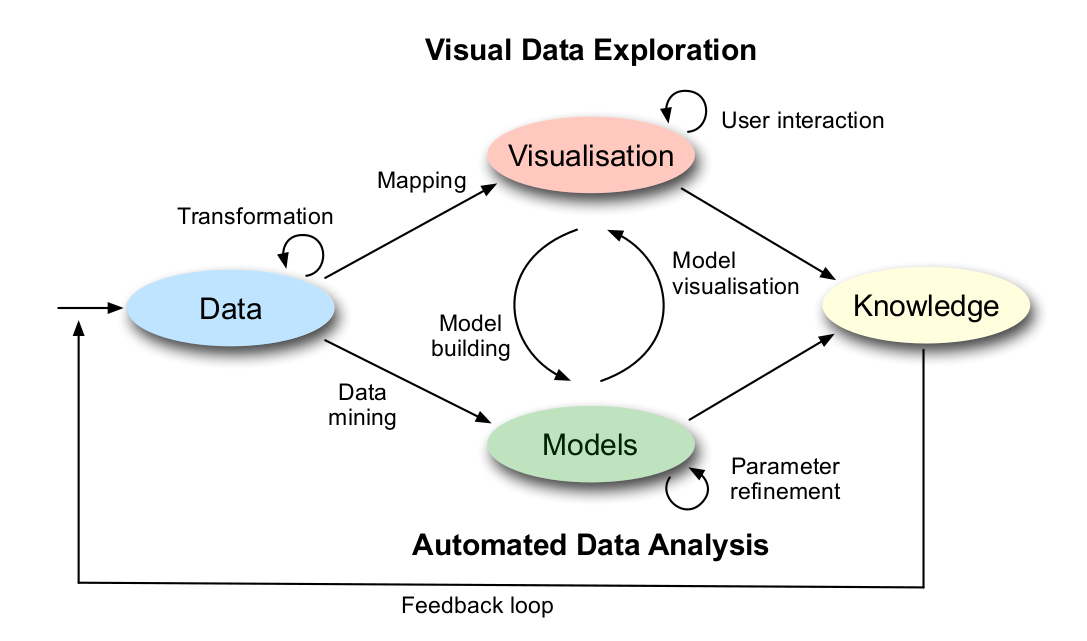
\includegraphics[height=5cm,keepaspectratio]{images/basics/va-process.png}
\caption[
    The visual analytics process is characterised through interaction between data, visualisations, models about the data and the users in order to discover knowledge \iacite{Keim2010}.
]{The visual analytics process is characterised through interaction between data, visualisations, models about the data and the users in order to discover knowledge.}
\label{fig:va-process}
\end{figure}

Figure \ref{fig:va-related} on page \pageref{fig:va-related} shows the interdisciplinary of visual analytics. With visualization as its core, other disciplines like data management, data analysis and data mining are close related and seem kind of obvious based on the knowledge of the visual analytics process and the definition of the term itself.

\begin{figure}[!htb]
\centering
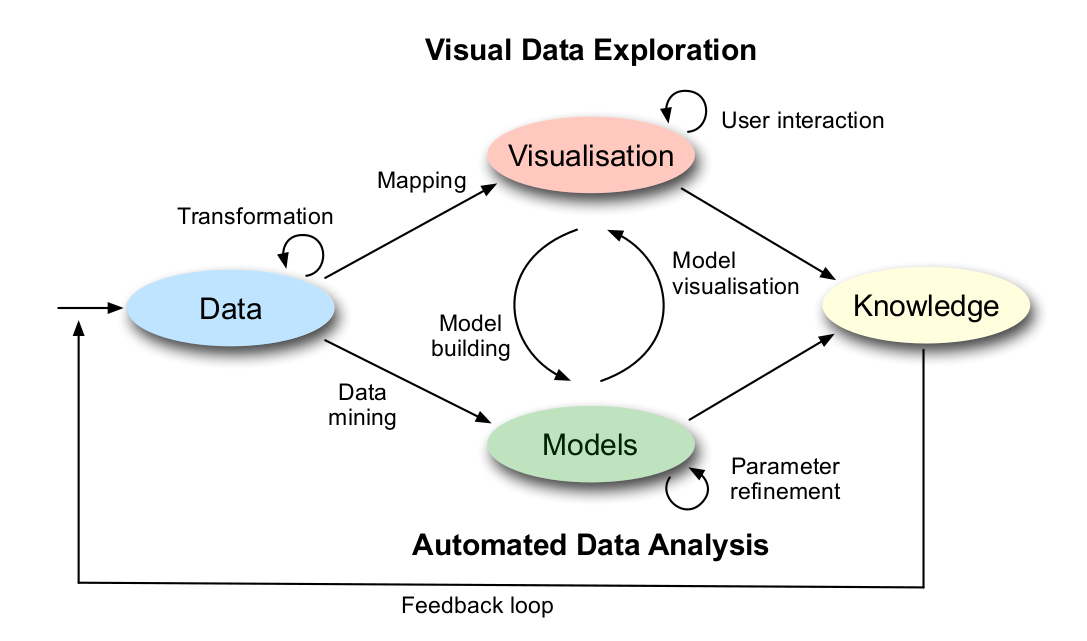
\includegraphics[height=5cm,keepaspectratio]{images/basics/va-process.png}
\caption[
    Visual analytics with core adjacent disciplines \iacite{Keim2010}.
]{Visual analytics with core adjacent disciplines.}
\label{fig:va-related}
\end{figure}

